\documentclass[12pt]{article}
\usepackage[margin=2.5cm]{geometry}
\usepackage{titling}
\usepackage{enumerate}
\usepackage{graphicx}
\usepackage{mdframed}
\usepackage{listings}
\usepackage{xcolor}
\usepackage{hyperref}
\usepackage[utf]{kotex}

\definecolor{codegreen}{rgb}{0,0.6,0}
\definecolor{codegray}{rgb}{0.5,0.5,0.5}
\definecolor{codepurple}{rgb}{0.58,0,0.82}
\definecolor{backcolour}{rgb}{0.95,0.95,0.92}

\lstdefinestyle{mystyle}{
    backgroundcolor=\color{backcolour},
    commentstyle=\color{codegreen},
    keywordstyle=\color{magenta},
    numberstyle=\tiny\color{codegray},
    stringstyle=\color{codepurple},
    basicstyle=\ttfamily\footnotesize,
    breakatwhitespace=false,
    breaklines=true,
    captionpos=b,
    keepspaces=true,
    numbers=left,
    numbersep=5pt,
    showspaces=false,
    showstringspaces=false,
    showtabs=false,
    tabsize=1
}

\lstset{style=mystyle}

\predate{}
\postdate{}

\begin{document}
\title{Lab 4: Abstract Data Type Solution}
\date{}
\maketitle

\section*{3) Running timing experiments}
\begin{enumerate}[1.]
    \item Your first task is to open \textit{timequeue.py} and follow the instructions
    contained within it to complete the timing experiment.

    \begin{lstlisting}[language=Python,caption={task\_3\_q1\_solution.py},captionpos=b]
    ...
    def _setup_queues(qsize: int, n: int) -> List[Queue]:
        """Return a list of <n> queues, each of the given size."""
        # Experiment preparation: make a list containing <n> queues,
        # each of size <qsize>.
        # You can "cheat" here and set your queue's _items attribute directly
        # to a list of the appropriate size by writing something like
        #
        #     queue._items = list(range(qsize))
        #
        # to save a bit of time in setting up the experiment.

        queue_list = []

        i = 0
        while i < n:
            queue = Queue()
            queue._items = list(range(qsize))

            queue_list.append(queue)
            i += 1

        return queue_list


    def time_queue() -> None:
        """Run timing experiments for Queue.enqueue and Queue.dequeue."""
        # The queue sizes to try.
        # You can change these values if you'd like.
        queue_sizes = [10000, 20000, 40000, 80000, 160000]

        # The number of times to call a single enqueue or dequeue operation.
        trials = 200

        # This loop runs the timing experiment. It has three main steps:
        for queue_size in queue_sizes:
            #   1. Initialize the sample queues.
            queues = _setup_queues(queue_size, trials)

            #   2. For each one, calling the function "timeit", takes three
            #      arguments:
            #        - a *string* representation of a piece of code to run
            #        - the number of times to run it (just 1 for us)
            #        - globals is a technical argument that you DON'T need to
            #          care about
            time = 0
            for queue in queues:
                time += timeit('queue.enqueue(1)', number=1, globals=locals())

            #   3. Report the total time taken to do an enqueue on each queue.
            print(f'enqueue: Queue size {queue_size:>7}, time {time}')

        # TODO: using the above loop as an analogy, write a second timing
        # experiment here that runs dequeue on the given queues, and reports the
        # time taken. Note that you can reuse most of the same code.
        for queue_size in queue_sizes:
            queues = _setup_queues(queue_size, trials)

            time = 0
            for queue in queues:
                time += timeit('queue.dequeue()', number=1, globals=locals())

            #   3. Report the total time taken to do an enqueue on each queue.
            print(f'dequeue: Queue size {queue_size:>7}, time {time}')
    ...
    \end{lstlisting}

    \item After you’ve run your experiment, you should notice that your two queue
    operations \textit{enqueue} and \textit{dequeue} behave quite differently.

    \bigskip

    While one seems to take the same amount of time no matter how many items are
    in the queue, the other takes longer and longer as the number of items are in
    the queue.

    \bigskip

    Compare your notes with other groups.
    Which end of a Python list seems to be the “slow” end? Do you have a guess
    as to why this might be the case? (If you don't: don't worry! You'll learn
    about this in later weeks.)

    \bigskip

    \begin{itemize}
        \item

        The front end of a Python list is the slow end.

        \bigskip

        This is because when \textit{LIST.pop(0)} is used, all of the later elements
        need to be shifted to the left by 1 position.

        \bigskip

        \begin{center}
        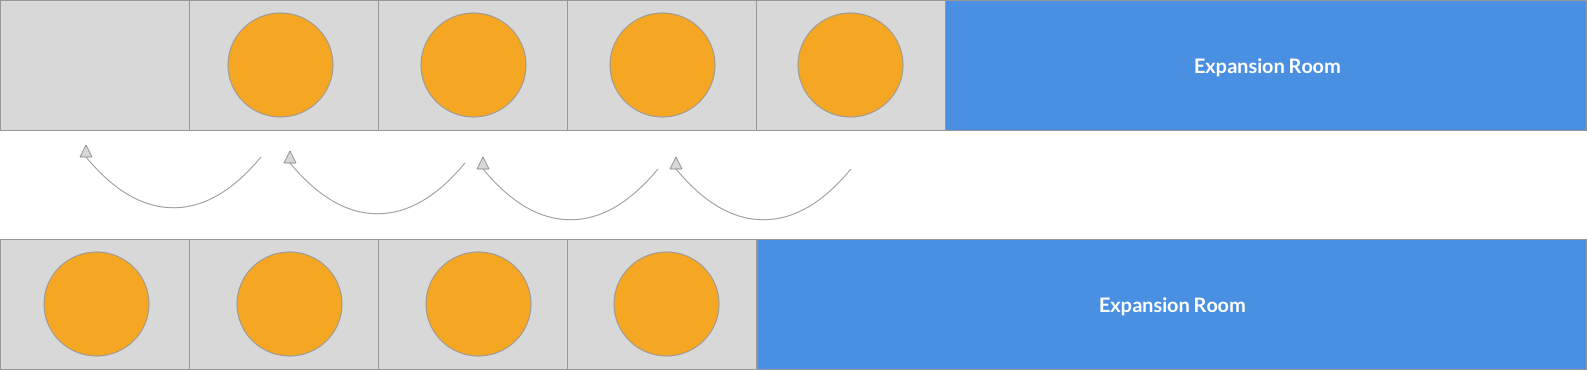
\includegraphics[width=0.8 \linewidth]{../../images/lab4_t3_q3_solution.png}
        \end{center}

    \end{itemize}

\end{enumerate}

\end{document}
